\documentclass{report}
\usepackage{booktabs, tabularx, caption, float, graphicx}

\begin{document}

\section{Introduction}
For this CA I will be investigating the AT\&T stock prices data set.
I will be aiming to answer the following question: Can I predict the future price of a stock based on a time series of previous stock data?
This time series will not contain all of the data from the previous time periods and the specific data that will be used will be chosen as part of my hyper-parameter selection.
The data for the stock prices has come from Kaggle and contains stock data for AT\&T between the years 2000 and 2020.

\section{Methodology and Data set}
Some of the key data in this data set are: The date (DATE)
The volume of the stock (VOL), this is the number of shares that were traded on that day. If a stock has a high volume then it means that shares for that stock changed hands a lot.
Opening price (OPENPRC), this is the value that the stock was first traded at on that day.
The asking high (ASKHI), this is the highest asking price for the stock on that day. The asking price of a seller is the lowest price that they will sell their share for. This makes the ASKHI the theoretical maximum that the stock was worth that day.
The lowest bid on the stock (BIDLO), this is the lowest bid that was put on the stock on that day. A bid is the highest price that someone is willing to pay for the stock. This makes the BIDLO the theoretical minimum a stock was worth that day.
the closing price of the stock (PRC). this is the final price that the stock was traded at during the day.
An interesting combined data point that could be included is the liquidity of the stock, this could be calculated using the ASKHI and the BIDLO and is a representation of how volatile the price of the stock is. It may also be useful for combining the ASKHI and BIDLO data into just one input which could increase regularisation and prevent overfitting of our models.

these are the data points that will be the most useful when we are trying to predict a stock's future values.
When we are creating a model for predicting the future of the stock we don't have to worry about things in this data set like:
PERMNO which is just a unique identification number for the shares that are being traded, this will be the same over all the data points and so is useless to include in our model.
The same justification can be used to remove the company name (COMNAM), TICKER, CUSIP, NCUSIP, PERMCO, SHRCD, ISSUNO, EXCHCD, SICCD, HSICCD, PRIMEXCH, TRDSTAT, SECSTAT

the following data points are not complete for all entries but when they are present they are identical across all entries and will therefore be discarded for this research question: SHRCLS, HSICMG, HSICIG, NAMEENDT, TSYMBOL NAICS
Another hyper-parameter that we can adjust in our model is how many time steps back we feed it to get our predictions. it will be interesting to see how it changes given more data and possibly at what point more data stops improving the model.

%liquidity: the difference between the ASKHI and the BIDLO could be a useful thing to have when predicting stock prices

for this project, I have identified the important data to be DATE, VOL, OPENPRC, ASKHI, BIDLO, PRC and liquidity. This is because they are the features that impact how much the stock is going to be traded at and they are all complete sets of data for all of the stock price snapshots. In the project, however, I will reduce the number down further to try and create a more regularised model as we don't want to include the data if it doesn't actually end up contributing much to our model.

\section{Results}

After investigating the Liquidity of the stocks I have found that even though the BIDLO and ASKHI have a very strong positive correlation to the stock price the liquidity does not have much correlation (0.3262 Pearsons coefficient, shown in Figure \ref{fig:LIQ}) and so may not offer as much information as including the ASKHI and BIDLO.

\begin{figure}
    \caption{Liquidity of stock against the price of stock}
    \centering
    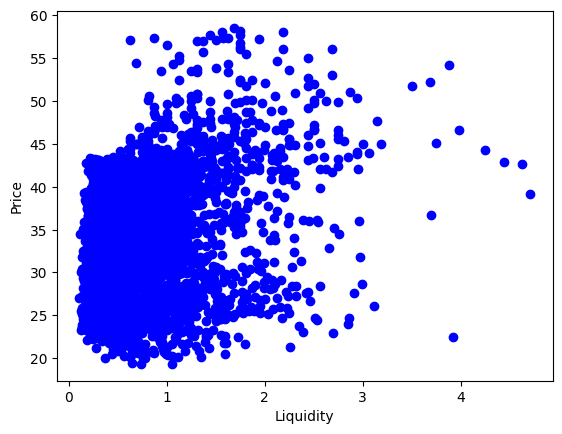
\includegraphics[scale=0.5]{LIQ.png}
    \label{fig:LIQ}
\end{figure}

For this project, I have used Linear regression and Lasso regression and Ridge regression to investigate the impact of stronger regularisation on my research question.
For my initial model, I had chosen to include all the data that i have deemed important in the section above for 5 previous days on the time series. This resulted in accurate predictions for just 1 day into the future. This was also the case with both ridge and lasso regression with linear and ridge regression having almost identical mean squared error and lasso falling just a little behind

\begin{minipage} {\linewidth}
\bigskip
\centering
\captionof{table}{Means Squared Error for predictions 1 day into the future using all important data}
\begin{tabular}{c c}
    Algorithm & MSE \\
    Linear Regression & 0.3135 \\
    Lasso Regression & 0.3994 \\
    Ridge Regression & 0.3135
\end{tabular}
\bigskip
\end{minipage}

For the next set of models, I removed some of the data and only left what I thought would be the most impactful for predicting the future price of the stock.
This was PRC VOL and LIQ (liquidity).
Doing this did not improve my results for any of the models when compared to using all of the available data but it did not make it significantly worse and offers a more general model so it will be what i use moving forward.

\begin{minipage} {\linewidth}
\bigskip
\centering
\captionof{table}{Means Squared Error for predictions 1 day into the future using all important data}
\begin{tabular}{c c}
    Algorithm & MSE \\
    Linear Regression & 0.3143 \\
    Lasso Regression & 0.4102 \\
    Ridge Regression & 0.3143
\end{tabular}
\bigskip
\end{minipage}

Predicting one day into the future isn't very useful to us as the timeframe is so short that we can reasonably predict one day ourselves. This means that we have to extrapolate further if we want to have our model be more useful.
With this further extrapolation comes more error in our model.
When increasing the time frame we still see that linear and ridge regression perform very similarly with lasso regression falling slightly behind however, this time there is an order of magnitude more error than from our one-day predictions
At this point, I also investigated the effects of increasing the number of previous points that we use. I used a 2 week period instead of a five-day period but that did not produce significantly better results.

\begin{minipage} {\linewidth}
\centering
\small
\setlength\tabcolsep{2pt}
\bigskip
\captionof{table}{Means Squared Error for predictions 1 day into the future using all important data}
\resizebox{1 \textwidth}{!} {
\begin{tabular}{c | c | c | c}
    Algorithm & MSE 10 days (5 previous points) & MSE 100 days (5 previous points) & MSE 100 days (14 previous points) \\
    Linear Regression & 2.6592, & 16.8129 & 17.0435 \\
    Lasso Regression & 2.7783 & 16.7768 & 16.9155 \\
    Ridge Regression & 2.6591 & 18.3947 & 17.0175
\end{tabular}
}
\bigskip
\end{minipage}

\begin{figure}
    \caption{Linear Regression predicting 10 days into the future}
    \centering
    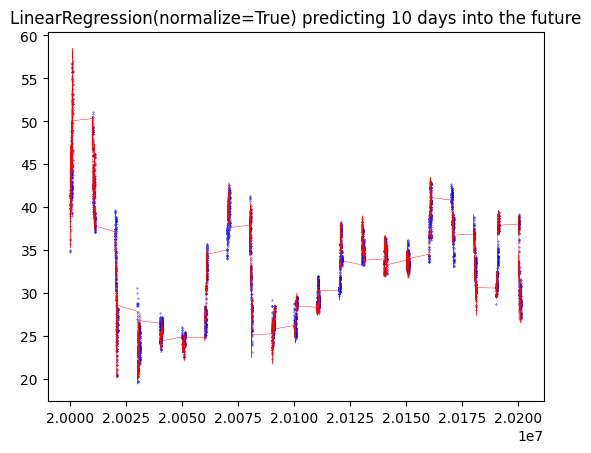
\includegraphics[scale=0.5]{10_day_regression.png}
    \label{fig:regression}
\end{figure}

You can see how the accuracy changes when extrapolating further in Figure \ref{fig:extrapolation}

\begin{figure}
    \caption{Plot of MSE based on time series length}
    \centering
    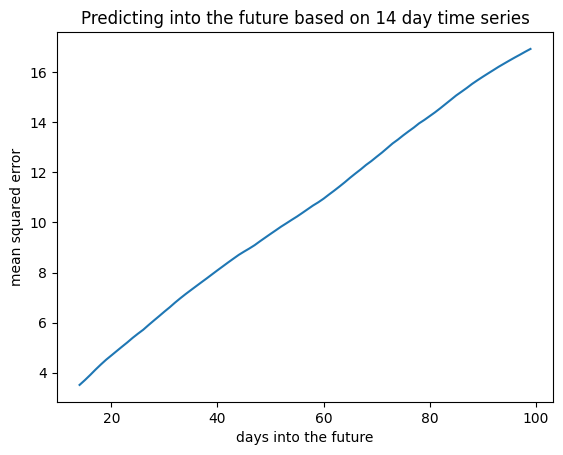
\includegraphics[scale=0.5]{predicting_into_future_plot.png}
    \label{fig:extrapolation}
\end{figure}

I also tried making predictions based on more of the time series, i tried using a two-week period of the time series instead of five days. This did not produce results that were significantly better.

You can see the effects of changing how far back we plot in Figure \ref{fig:vary_time_series_length}

\begin{figure}
    \caption{Plot of MSE based on time series length}
    \centering
    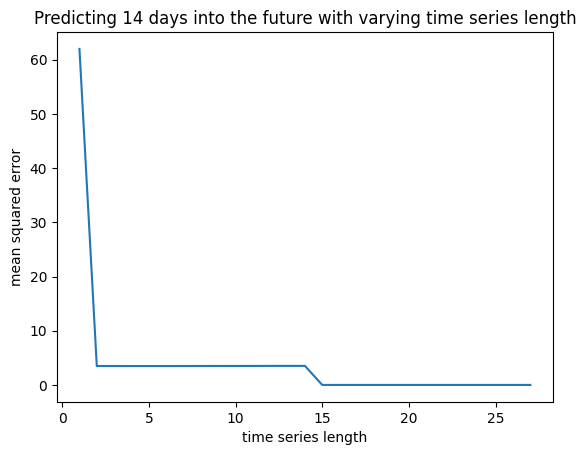
\includegraphics[scale=0.5]{varying_length_plot.png}
    \label{fig:vary_time_series_length}
\end{figure}

Overall for this data set, it seems as though linear regression performs the best for predicting future values across the board and so that would have to be the model that I would recommend. Although ridge regression was a close second and offers more regularisation in your model and so in a different data set could be a better choice and is definitely worth trying.
For this data set Lasso regression performed quite poorly, especially when using normalized data as the accuracy of Lasso regression became unusably bad. (~48 MSE when predicting one day into the future).
Overall I think these models are accurate when you are not extrapolating too far. The results for the predictions 10 days into the future are not too erroneous and could be used. However, once you start predicting 100 days your error is too large to use. Even though the error for each prediction would be about 4 units the data we are trying toA predict for was generally between 25 and 55 units making these errors quite large proportionally.

\section{Discussion}

To conclude I think that we can predict the future price of the stock based on the time series, however, this has limitations. The major limitation is the fact that if we want our data to be more useful to us we have to extrapolate further which leads to more errors in our predictions and a less reliable model.

The next step in analysing this data set would be to try a different type of model, perhaps a neural network would be able to capture something in the data that would help the model to predict further into the future with more accuracy and maybe allow for more complex relationships between features as the linear methods that have been used here are limited in the ways that the features can interact with each other. Something like a Multi-Layer perceptron neural network would be able to extract more complex relationships.

\end{document}
